% !TEX TS-program = pdflatex
% !TEX encoding = UTF-8 Unicode

\documentclass[11pt]{article}

\usepackage[utf8]{inputenc} % set input encoding (not needed with XeLaTeX)

\usepackage{geometry} % to change the page dimensions
\geometry{a4paper} % or letterpaper (US) or a5paper or....


\usepackage{longtable}
\usepackage{booktabs} % for much better looking tables
\usepackage{array} % for better arrays (eg matrices) in maths
\usepackage{paralist} % very flexible & customisable lists (eg. enumerate/itemize, etc.)
\usepackage{verbatim} % adds environment for commenting out blocks of text & for better verbatim
\usepackage{subfig} % make it possible to include more than one captioned figure/table in a single float

\usepackage{authblk}
\usepackage{amssymb}
\usepackage{amsthm}
\usepackage{amsmath}
\usepackage[pdfstartview=FitH]{hyperref}
\usepackage{graphicx} % support the \includegraphics command and options
\usepackage{parskip}
\usepackage{setspace}
\setstretch{ 1.5 }

%%% HEADERS & FOOTERS
\usepackage{fancyhdr} % This should be set AFTER setting up the page geometry
\pagestyle{fancy} % options: empty , plain , fancy
\renewcommand{\headrulewidth}{0pt} % customise the layout...
\lhead{}\chead{}\rhead{}
\lfoot{}\cfoot{\thepage}\rfoot{}

%%% SECTION TITLE APPEARANCE
%\usepackage{sectsty}
%\allsectionsfont{\sffamily\mdseries\upshape} % (See the fntguide.pdf for font help)
% (This matches ConTeXt defaults)

%%% ToC (table of contents) APPEARANCE
%\usepackage[nottoc,notlof,notlot]{tocbibind} % Put the bibliography in the ToC
%\usepackage[titles,subfigure]{tocloft} % Alter the style of the Table of Contents
%\renewcommand{\cftsecfont}{\rmfamily\mdseries\upshape}
%\renewcommand{\cftsecpagefont}{\rmfamily\mdseries\upshape} % No bold!

\def\tightlist{}

\title{ Topaze Publishing \\ \large A Python / Pandoc based publishing system \\ v1.0}

\author{
   Stefan Loesch \\
  \texttt{\href{mailto:stefan@topaze.blue }{ stefan@topaze.blue }}    
  \and
  Oscar D Torson \\
  \texttt{\href{mailto:oscar@topaze.blue }{ oscar@topaze.blue } }
}

\affil{  \href{  }{  }  }
%\date{} % Activate to display a given date or no date (if empty),
         % otherwise the current date is printed 

\setlength{\parindent}{0pt}

\begin{document}

\maketitle

\begin{abstract}
   Topaze Publishing ("TP") is a collection of Python libraries destined to create
beautiful and modular papers, mostly from augmented markdown sources, ie markdown 
files with a yaml header for metadata. The python libraries mostly deal with the 
creation of the aggregated and augmented markdown file, and possibly its conversion
to html. They then invoke pandoc for conversion into other formats, including Word,
LaTeX and ultimately pdf.

\end{abstract}

\pagebreak

\tableofcontents

\pagebreak






\pagebreak

\hypertarget{section-overview}{%
\section{Section: Overview}\label{section-overview}}


\pagebreak

\hypertarget{introduction}{%
\subsection{Introduction}\label{introduction}}


This document is mostly a destined to show the different options of how
documents can be created. Before we have a look at the document so far
we briefly want to mention how documents are created: key to this is
\texttt{Convert.py} in the \texttt{code} directory, or
\texttt{Convert.ipynb}. Those two files are equivalent and kept in synch
by JupyText. Note that whilst \texttt{Convert.py} can be run in a Python
interpreter it will fail if not run in a proper Jupyter environment as
we are using the bang-execution framework, eg \texttt{!pandoc} to
execute pandoc.

Up to here we have already seen the following features

\begin{itemize}
\item
  documents are assembled according to their tags; eg
  \texttt{tags:\ DocPaper} unites all the documents that are part of
  DocPaper; the files are assembled in lexical order, hence the prefix
  \texttt{000} or \texttt{t000}; a file with
  \texttt{tags:\ DocPaper,\ OtherPaper} would be part of both papers
\item
  the document-wide metadata (in \texttt{000}) that in particular sets
  key frontmatter items like \texttt{title}, \texttt{subtitle},
  \texttt{abstract}, \texttt{author(s)}, \texttt{date} and
  \texttt{version}; it also contains key LaTeX items under the
  \texttt{latex} key (see below)
\item
  a custom title page (in \texttt{010}), to be used for non-tex
  documents only (\texttt{notex:\ true}); it is a template
  (\texttt{istemplate:\ true}) which means that eg \texttt{\{title\}}
  will be replaced with the document title; tex documents
\item
  two structure pages (in \texttt{100}, \texttt{101}), here specifically
  a section break (\texttt{type:\ section}) and a chapter break
  (\texttt{type:\ chapter}); a page break is included before
  (\texttt{breakbefore:\ 1}; this may or may not work in LaTeX)
\end{itemize}

The aforementioned items under the \texttt{latex} key are as follows:

\begin{itemize}
\tightlist
\item
  \texttt{template}: which template to use (the templates are in
  \texttt{code/templates})
\item
  \texttt{fontsizea}: eg \texttt{11pt}
\item
  \texttt{geometry}: eg \texttt{a4paper}
\item
  \texttt{stretch}: eg \texttt{1.5} for line spacing
\end{itemize}

The first feature we see in this paper the \texttt{WordTag} feature
where we include raw XML into the markdown that pandoc in term preserves
in the generated Word documents (it ignores it when producing LaTeX).
Wordtags are included with the following syntax

\begin{verbatim}
<!--WT=[ITEM]-->
\end{verbatim}

where ITEM can be any of

\begin{itemize}
\tightlist
\item
  \texttt{PAGEBREAK}
\item
  \texttt{SECTIONBREAK}
\end{itemize}

Other tags are planned, but have not been introduced yet. The code for
this is in \texttt{wordtags.py}.

We can also include equations into the markdown, that pandoc then
properly converts to Word (or to LaTeX, but this is trivial). Equations
can be included literally, eg like here

\[
E = mc^2
\]

We are also providing a module (in \texttt{formulalib.py}) that allows
to include formulas generated in Python via Sympy, typically in a
Jupyter notebook (or in multiple Jupyter notebooks) that can be reused
across multiple documents. Below is an example for an included equation

\[
a^{2} + b^{2} = c^{2}
\]

We can also include images using the markdown \texttt{!{[}{]}()}
construct. In Word, those images will appear exactly where they have
been placed. In LaTeX, they will float and the text in \texttt{{[}.{]}}
will be the figure caption that can be used to refer to them in the
text.

\begin{figure}
\centering
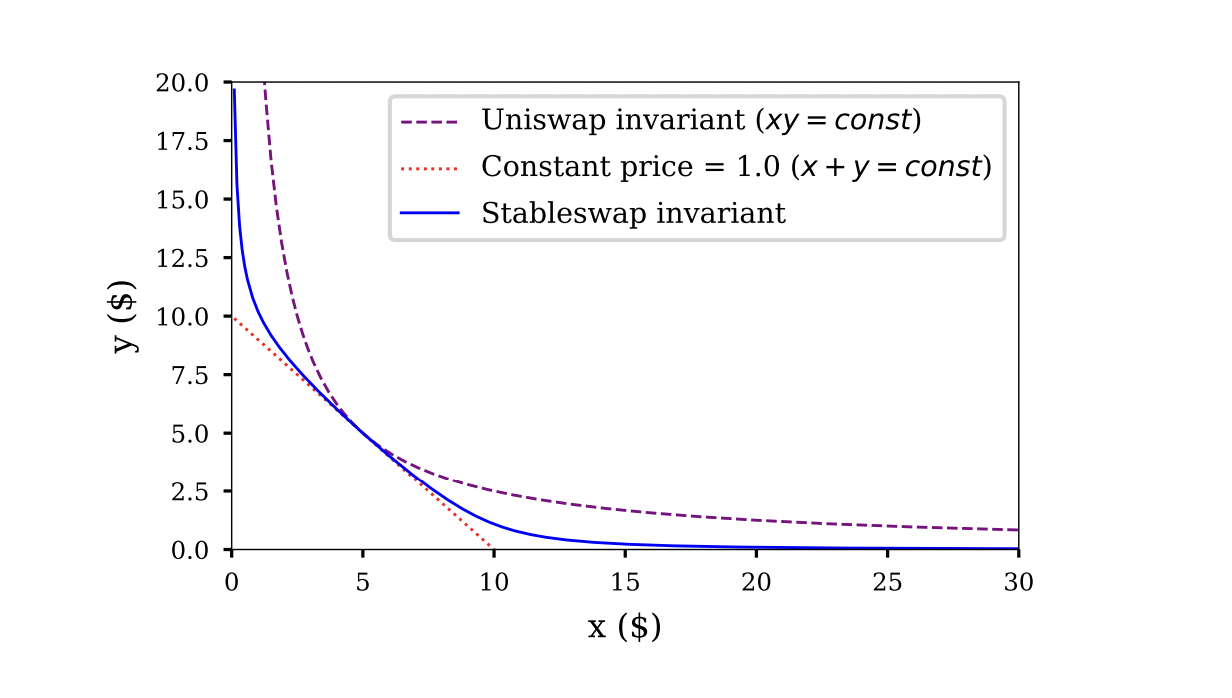
\includegraphics[width=10cm,keepaspectratio]{_img/016-Chart01.png}
\caption{Example Image}
\end{figure}

In Word this text is after the image. In LaTeX, it will have the caption
``Example Image'', but to where it will float is rather uncertain. Note
that images will have to be in the \texttt{src/\_img} (which means
they'll show up in VSCode linked preview) and Convert will copy them to
\texttt{out/\_img}. ATTENTION: \texttt{out/\_img} will be cleaned up
before every run. Do not store images there.


\hypertarget{after-a-section-break}{%
\subsection{After a section break}\label{after-a-section-break}}

The above heading is preceded by a
\texttt{\textless{}!-\/-wt=SECTIONBREAK-\/-\textgreater{}}. Now let's do
some lorem ipsum dolor sit amet, consectetur adipiscing elit. Nulla eu
congue nulla. Nulla congue vel quam vitae convallis. Proin finibus
congue orci eu ultricies. Curabitur tristique et justo eu fringilla.

\begin{quote}
Praesent tincidunt tellus sit amet leo euismod efficitur. Pellentesque
habitant morbi tristique senectus et netus et malesuada fames ac turpis
egestas. Vestibulum in turpis sed leo tincidunt dictum quis eu mi. Sed
molestie ligula eget dignissim viverra.
\end{quote}

Ut pulvinar lorem sit amet metus condimentum bibendum. Vestibulum
egestas ut erat sed scelerisque. Aliquam eget lectus sit amet eros
dignissim dapibus. Phasellus quis orci diam. Pellentesque et tempus
tortor. Duis mollis efficitur nisi nec commodo. Vestibulum bibendum
risus id diam ultricies congue. Vivamus et mollis lectus.

\begin{itemize}
\item
  Suspendisse fringilla erat enim, id iaculis eros ultricies et. Fusce
  consectetur nisi vel venenatis tincidunt. Aenean cursus ante ut
  accumsan fringilla.
\item
  Nam posuere quam a feugiat varius. Curabitur ullamcorper vehicula
  justo sit amet convallis.
\item
  Proin a nisl ut elit fringilla maximus sollicitudin ac libero.
  Maecenas molestie diam sem, vitae ultricies magna efficitur sed.
\end{itemize}

Aliquam erat volutpat. Maecenas vehicula augue purus, a dapibus justo
accumsan non. Phasellus faucibus finibus tristique. Duis cursus
porttitor nibh. Aliquam nec est metus. Ut eu lacus in ante luctus
volutpat. Nulla eget tincidunt quam, nec semper arcu. Nulla arcu massa,
posuere non leo eu, mollis egestas ligula.

\hypertarget{after-a-page-break}{%
\subsubsection{After a page break}\label{after-a-page-break}}

The above heading is preceded by a
\texttt{\textless{}!-\/-wt=PAGEBREAK-\/-\textgreater{}}. More of the
lorem ipsum pellentesque consequat malesuada erat sit amet aliquam. Ut
mattis arcu nec ipsum luctus, et auctor eros cursus. Curabitur varius
vulputate purus, non eleifend dui dapibus vel. Quisque eleifend massa
vel nulla convallis luctus. Etiam dignissim vel diam quis commodo.

Nulla tristique nulla ut arcu iaculis, ac tempus sapien laoreet. Quisque
et dui sit amet mi dapibus aliquet. Nam sit amet lectus quis urna
venenatis mattis. Morbi mattis, diam vehicula gravida iaculis, ante eros
maximus neque, a tristique nunc sapien sit amet leo.

\begin{verbatim}
In hac habitasse platea dictumst.
Vestibulum eu ligula at sapien tincidunt.
Interdum et malesuada fames ac ante.
Ipsum primis in faucibus fusce.
\end{verbatim}

Nam ut interdum risus, nec feugiat nisl. Sed vestibulum dui eget aliquam
dictum. Phasellus imperdiet sem massa. Integer tincidunt nisi elit, eget
consequat mauris tristique id.

\hypertarget{after-another-page-break}{%
\subsubsection{After another page
break}\label{after-another-page-break}}

The above heading is preceded by a
\texttt{\textless{}!-\/-wt=BREAK:page-\/-\textgreater{}}. More lorem
ipsum dolor sit amet, consectetur adipiscing elit. Proin at lobortis
orci, quis rhoncus ipsum. Nam vitae diam vel nisl euismod bibendum.
Mauris a odio nisi. Mauris vestibulum eu arcu sodales efficitur. Vivamus
sagittis varius turpis sed accumsan. Nunc interdum nunc vel tellus
mattis, ut suscipit elit varius. Etiam sed diam sem.

\begin{enumerate}
\def\labelenumi{\arabic{enumi}.}
\item
  Vestibulum in diam eget metus tristique vestibulum. Integer semper
  purus in ultricies cursus. Duis malesuada sagittis arcu, at consequat
  tortor iaculis ut. Nam id est nunc.
\item
  In odio magna, cursus ac tempus et, mollis ac metus. Nulla bibendum
  est mollis, auctor tellus eget, hendrerit felis. Cras malesuada
  blandit ante, id rhoncus nunc efficitur non.
\item
  Quisque condimentum efficitur ligula, a molestie tortor mollis in.
  Nunc vulputate malesuada felis. Pellentesque pellentesque, orci vitae
  bibendum malesuada, ipsum neque facilisis eros, non dignissim felis
  lectus id elit. Nullam tincidunt elit commodo luctus suscipit.
\item
  Integer accumsan fringilla mi, a tempus diam. Nullam erat sapien,
  posuere et orci in, convallis tincidunt velit. Fusce tincidunt dictum
  libero, vitae tincidunt sapien bibendum eget.
\end{enumerate}

Nunc ac egestas neque. Donec consequat viverra nunc a mattis. Phasellus
finibus lorem id pulvinar tincidunt. Nulla vestibulum placerat eros ut
interdum. Aliquam accumsan hendrerit augue, eget fermentum sem volutpat
vitae. Aliquam volutpat scelerisque lorem. Sed ultricies, felis vitae
pharetra tempus, nunc erat ornare metus, sed placerat nibh mi vel
mauris.


\hypertarget{equation-testing}{%
\subsection{Equation testing}\label{equation-testing}}

This sections is testing equation tags of the form
\texttt{\$\$!=ERROR{[}...{]}=\$\$}

Lorem ipsum dolor sit amet, consectetur adipiscing elit. Integer sit
amet enim vitae nibh commodo tincidunt. Nam et felis enim. Etiam blandit
et neque et faucibus. Pellentesque habitant morbi tristique senectus et
netus et malesuada fames ac turpis egestas. Sed sed vestibulum mauris,
vitae ultrices odio. Maecenas sodales porta ex, et dapibus ante eleifend
vel.

\[
a^{2} + b^{2} = c^{2}
\]

The above equation has no namespace, hence the ID is
\texttt{PythagorasE}.

Sed tempus mi viverra suscipit ultrices. Ut finibus tortor risus, quis
dictum nisi gravida quis. Donec malesuada velit vitae aliquet dignissim.
Vestibulum ante ipsum primis in faucibus orci luctus et ultrices posuere
cubilia curae; Sed ut mauris ante. Mauris et maximus ante, blandit
elementum lacus. Donec sagittis nibh tortor, at commodo nibh commodo ac.

\[
b = - \sqrt{- a^{2} + c^{2}}
\]

This equation is imported from the second notebook, and as there were
overlapping names we prefaced the import in \texttt{Context.py} with the
\texttt{f2} namespace, so the ID of this equation is
\texttt{f2.PythagorasBE}.

The code in \texttt{Context.py} reads as follows

\begin{verbatim}
# import formulas without namespace
from src.TestFormulas1 import FORMULAS    

# import formulas into temp location...                  
from src.TestFormulas2 import FORMULAS as _FORMULAS2 

# ...and add them with namespace f2       
FORMULAS.addfrom(_FORMULAS2, ns="f2")                       
\end{verbatim}

Aenean feugiat vulputate odio id gravida. Praesent ac tellus sed tellus
varius sodales non eu lacus. Donec venenatis metus eget turpis accumsan
varius. Vestibulum bibendum leo non malesuada porta. Donec condimentum
tempus dolor vel rutrum. Ut et quam rutrum, volutpat orci at, pharetra
diam.

Here we show the same equation ID (and incidentally the same equation,
but that does not necessarily have to be the case) using two different
namespaces.

\[
E = c^{2} m
\]

Nulla vitae mauris nisi. Morbi nec neque sodales ipsum malesuada
fringilla. Quisque rhoncus at nisi eget commodo. Donec rutrum at ipsum a
pellentesque. Nullam porta pulvinar elementum. Integer et magna lectus.
Quisque vulputate ligula in sapien venenatis auctor.

\[
E = c^{2} m
\]

Aenean a volutpat quam, ac ultrices nisl. Nam laoreet ex nec orci
elementum, ut mattis justo venenatis. Cras mi velit, aliquet eu quam
imperdiet, tincidunt sodales ipsum.


\hypertarget{working-with-templates}{%
\section{Working with templates}\label{working-with-templates}}

In this file we are working with templates. For this to work we need
\texttt{istemplate:\ true}. The metadata section of this file reads as
follows

localmeta1: my local meta data item 1 localmeta2: my local meta data
item 2

data: localdata1: my local data item 1 localdata2: my local data item 2

\hypertarget{example-template-evaluations}{%
\subsection{Example template
evaluations}\label{example-template-evaluations}}

\begin{itemize}
\item
  \textbf{localmeta1} from local meta data "\{\_m{[}localmeta1{]}\}" (it
  does \textbf{not} appear in the global data!)
\item
  \textbf{localdata2} from the local data "\{\_d{[}localdata2{]}\}" and
  from the global data "\{\_d{[}localdata2{]}\}" (because it only
  appears in this file) and from the global data using kwargs
  ``\{localdata2\}''
\item
  \textbf{title} from global data (it is not defined in this file)
  "\{\_d{[}title{]}\}" and using kwargs ``\{title\}''
\item
  \textbf{authors} as a list ``\{authors\}''
\item
  the first author as dict ``\{authors{[}0{]}\}''
\item
  the second author nicely formatted ``\{authors{[}1{]}{[}name{]}\}
  \textless\{authors{[}1{]}{[}email{]}\}\textgreater{}''
\end{itemize}


\hypertarget{explaining-datas-and-templates}{%
\subsection{Explaining datas and
templates}\label{explaining-datas-and-templates}}

\hypertarget{data}{%
\subsubsection{Data}\label{data}}

Before we can understand templates, we need to understand what data is,
and how it is handled. There are two types of data in this system, meta
data (``metadata'') and data proper (``data''). The differences are as
follow

\begin{enumerate}
\def\labelenumi{\arabic{enumi}.}
\item
  \textbf{metadata}: metadata is local to a specific file, and whilst it
  can in principle be arbitrary data, it is mostly used to convey
  information about the file in question; for example, important
  metadata items are \texttt{tags} and \texttt{istemplate}, both of
  which being critical to how a specific file is treated
\item
  \textbf{data}: data is aggregated across all files into a single
  global dataset; the system does not make any further use of the data,
  other than providing it via the templating system as demonstrated
  above, and as explained below
\end{enumerate}

For \emph{regular files} (markdown etc), metadata is all data in the
preamble yaml section, \emph{except} the items that hang under the
\texttt{data} entry itself: all those are considered data. For example
the preamble of this file is as follows

\begin{verbatim}
tags: DocPaper

istemplate: true

localmeta1: my local meta data item 1
localmeta2: my local meta data item 2

data:
    localdata1: my local data item 1
    localdata2: my local data item 2
\end{verbatim}

The items \texttt{tags}, \texttt{istemplate} and \texttt{localmeta1/2}
are metadata, with the first two being actively considered by the
system. The items \texttt{localdata1} and \texttt{localdata2} are data,
and they will be aggregated across the entire system

In \emph{data file} (yaml extension), all data is considered data and
aggregated globally. For example below are the data items of this
document that, as we can see, contain information like the title and
subtitle as well as version and date

\begin{verbatim}
tags: DocPaper

version:  "0.0"
date:     "13 Oct 2022"

title:        Topaze Blue Advisory
subtitle:     Advising on anything Defi
\end{verbatim}

Note that technically the data for data files is also considered its
meta data as we see above with the data item \texttt{tags}. This is
somewhat inelegant as this means that the metadata of data files is also
subject to aggregation, but in the grand scheme of things we do not care
enough to change it.

\hypertarget{data-aggregation}{%
\subsubsection{Data aggregation}\label{data-aggregation}}

A final word on \textbf{data aggregation}: the way it works is that data
is collected in a single dict, starting from the front of the document
and working one's way through to the back. To the extent that there are
no duplicate keys this does not matter, but if there are the later data
replaces the earlier one. For structured data the result is undefined.
What we mean with this is the following. Consider the following data in
file 1

\begin{verbatim}
lorem:
ipsum:  1
dolor:  2
\end{verbatim}

and the following data in the later file 2

\begin{verbatim}
lorem:
  dolor:  20
  sit:    30
\end{verbatim}

In this case you can rely on the fact that the data from file 2 is
present, ie dolor is 20 and sit is 30. However -- you should not rely in
ipsum being present in the final data (but also not on it \emph{not}
being there; it is undefined).

\hypertarget{using-templates}{%
\subsubsection{Using templates}\label{using-templates}}

Templates are simple Python templates that are evaluated with
\texttt{.format}. More specfically, if we assume that the local metadata
and data are in \texttt{lm} and \texttt{ld} respectively, and the global
data is in \texttt{gd}, then the call to format is exectuted as follows

\begin{verbatim}
template.format(_m=lm, _ld=ld, _d=gd, **gd)
\end{verbatim}

This means that local meta data can be accesed in the template as
\texttt{\{\_m{[}item{]}\}} and local data as
\texttt{\{\_ld{[}item{]}\}}. Global data can be accessed either as
\texttt{\{\_d{[}item{]}\}} or simply as \texttt{\{item\}}. Note that
unless it is overwritten at a later stage, local data will be included
in the global dataset as well, so in most cases \texttt{\{item\}},
\texttt{\{\_d{[}item{]}\}} and \texttt{\{\_ld{[}item{]}\}} will be
equivalent.

Here also a short reminder that templates allow for accessing structured
data as well. For example, if \texttt{lst} is a list and \texttt{dct} is
a dict in the global data, then \texttt{\{lst{[}0{]}\}} gets the first
list item, and \texttt{\{dct{[}key{]}\}} accesses an element in the
dict. Hierarchical access works as expected, eg
\texttt{\{item{[}k1{]}{[}1{]}{[}k2{]}\}} would access and element that
is part of a dict that is part of a list that in turn is part of a dict.


\hypertarget{references}{%
\section{References}\label{references}}

\hypertarget{sympy-references}{%
\subsection{Sympy References}\label{sympy-references}}

\begin{itemize}
\tightlist
\item
  The general SymPy documentation is
  \href{https://docs.sympy.org/latest/index.html}{here}
\item
  A very interesting article about upgrading SymPy to allow for more
  elegant evaluation is
  \href{https://awstip.com/customizing-pythons-sympy-for-easy-equation-manipulation-ca30b9d0dabf}{here};
  the code is also on
  \href{https://github.com/mathcube7/customize-sympy/blob/main/customizer.py}{github}
\end{itemize}


\end{document}